\chapter{Lösung}
\label{chap:loesung}
% In diesem Kapitel beschreiben Sie Ihre Lösung des Problems. Geben Sie dem Leser genügend Einblick in die Lösung, so dass er Ihre Arbeit entsprechend würdigen kann. Verwenden Sie aber Anhänge für Dinge, die hier nicht unbedingt bis ins letzte Detail verstanden werden müssen.
Die Aufgabenstellung beschreibt das Ziel dieser Bachelor Thesis mit dem einfachen Satz ``Ziel dieser Arbeit ist die Entwicklung und Anwendung eines Systems zur Speicherung (von Daten) in einer semantischen Datenbank$\cdots$''.~\cite{Aufgabenstellung} Es sollen also Daten in einem Datenspeicher abgelegt werden. Der einzig unbekannte Faktor ist dabei, dass es sich bei der Datenbank um eine semantische Datenbank handeln soll. Bei genauerer Betrachtung wird interessierten Personen bewusst, das sich Einiges dahinter verbirgt.

Auf der einen Seite eine Ansammlung von neuen Technologien und Theorien. Auf der anderen Seite eine völlig unbekannte und vor allem ungewohnte Denkweise, welche erst erkannt und dann auch angewendet werden muss. Dies ist gerade für Personen aus der Informatik, speziell mit objektorientiertem Hintergrund eine Herausforderung. Die Erfahrungen und Schwierigkeiten dabei werden im~\autoref{sub:modellierung_der_ontologie} beschrieben.

Eine Anforderung, welche bei der Spezifikation der Meilensteine nicht erwähnt wurde, ist der Anspruch der Autoren innerhalb einer gewissen Wissensdomäne Fragen beantworten zu können. Dies impliziert bereits fundiertes Fachwissen der Thematik, da Fragen anhand der Semantik der Inhalte beantwortet werden sollen. 

Die Organisation sowie die Herangehensweise der Autoren wurden im \autoref{chap:administratives} und \autoref{chap:vorgehen} ausführlich beschrieben. In diesem Kapitel liegt der Fokus auf der tatsächlichen Lösung der Anforderungen.

\section{Von der Wissenserarbeitung zum Tutorial}
\label{sec:loesung_tutorial}
Um die oben erwähnten Technologien, Sprachen und Theorien zu erarbeiten und diese vor allem mit dem Leser zu teilen, wurde ein Tutorial erarbeitet. Dabei war es schwierig ein einfach nutzbares Tutorial zu erstellen, dem Leser dabei aber auch genügend Hintergrundwissen zu vermitteln. Der Leser soll wirklich verstehen können was hinter einer Wissensmodellierung respektive einem Expertensystem steckt. Daraus entstand ein Dokument, welches die Modellierung aus drei Perspektiven beleuchtet. Diese werden ausführlich im \autoref{subsec:dokumentation_wissensmodellierung_aufbau} beschrieben.

\section{Modellierung}
\label{sec:loesung_modellierung}

Semantische Datenbanken werden auf Basis von Ontologien gebildet. Eine Ontologie wird für eine Problemdomäne erstellt und bildet ihr Wissen ab. Die Problemdomäne dieser Arbeit ist das Reisen. Es wurde entschieden sich vorerst auf Ausflüge in der Schweiz zu begrenzen. Damit ist es möglich die Mächtigkeit eines Expertensystems aufzuzeigen. Die gesamte Modellierung wurde mithilfe von OWL formuliert. Bei OWL handelt es sich um eine Ontologieabbildungssprache. Benötigte Regeln werden in der Regelsprache SWRL formuliert. Details dazu können im Tutorial nachgelesen werden. TODO ref zu Tutorial

Zur Veranschaulichung wurde jeder Teil der Ontologie und die dazugehörigen Regeln in einem semantischen Netz abgebildet. Sämtliche Grafiken finden sich als Anhang TODO.

\begin{figure}[H]
\centering \rotatebox{0}{\scalebox{0.3}[0.3]{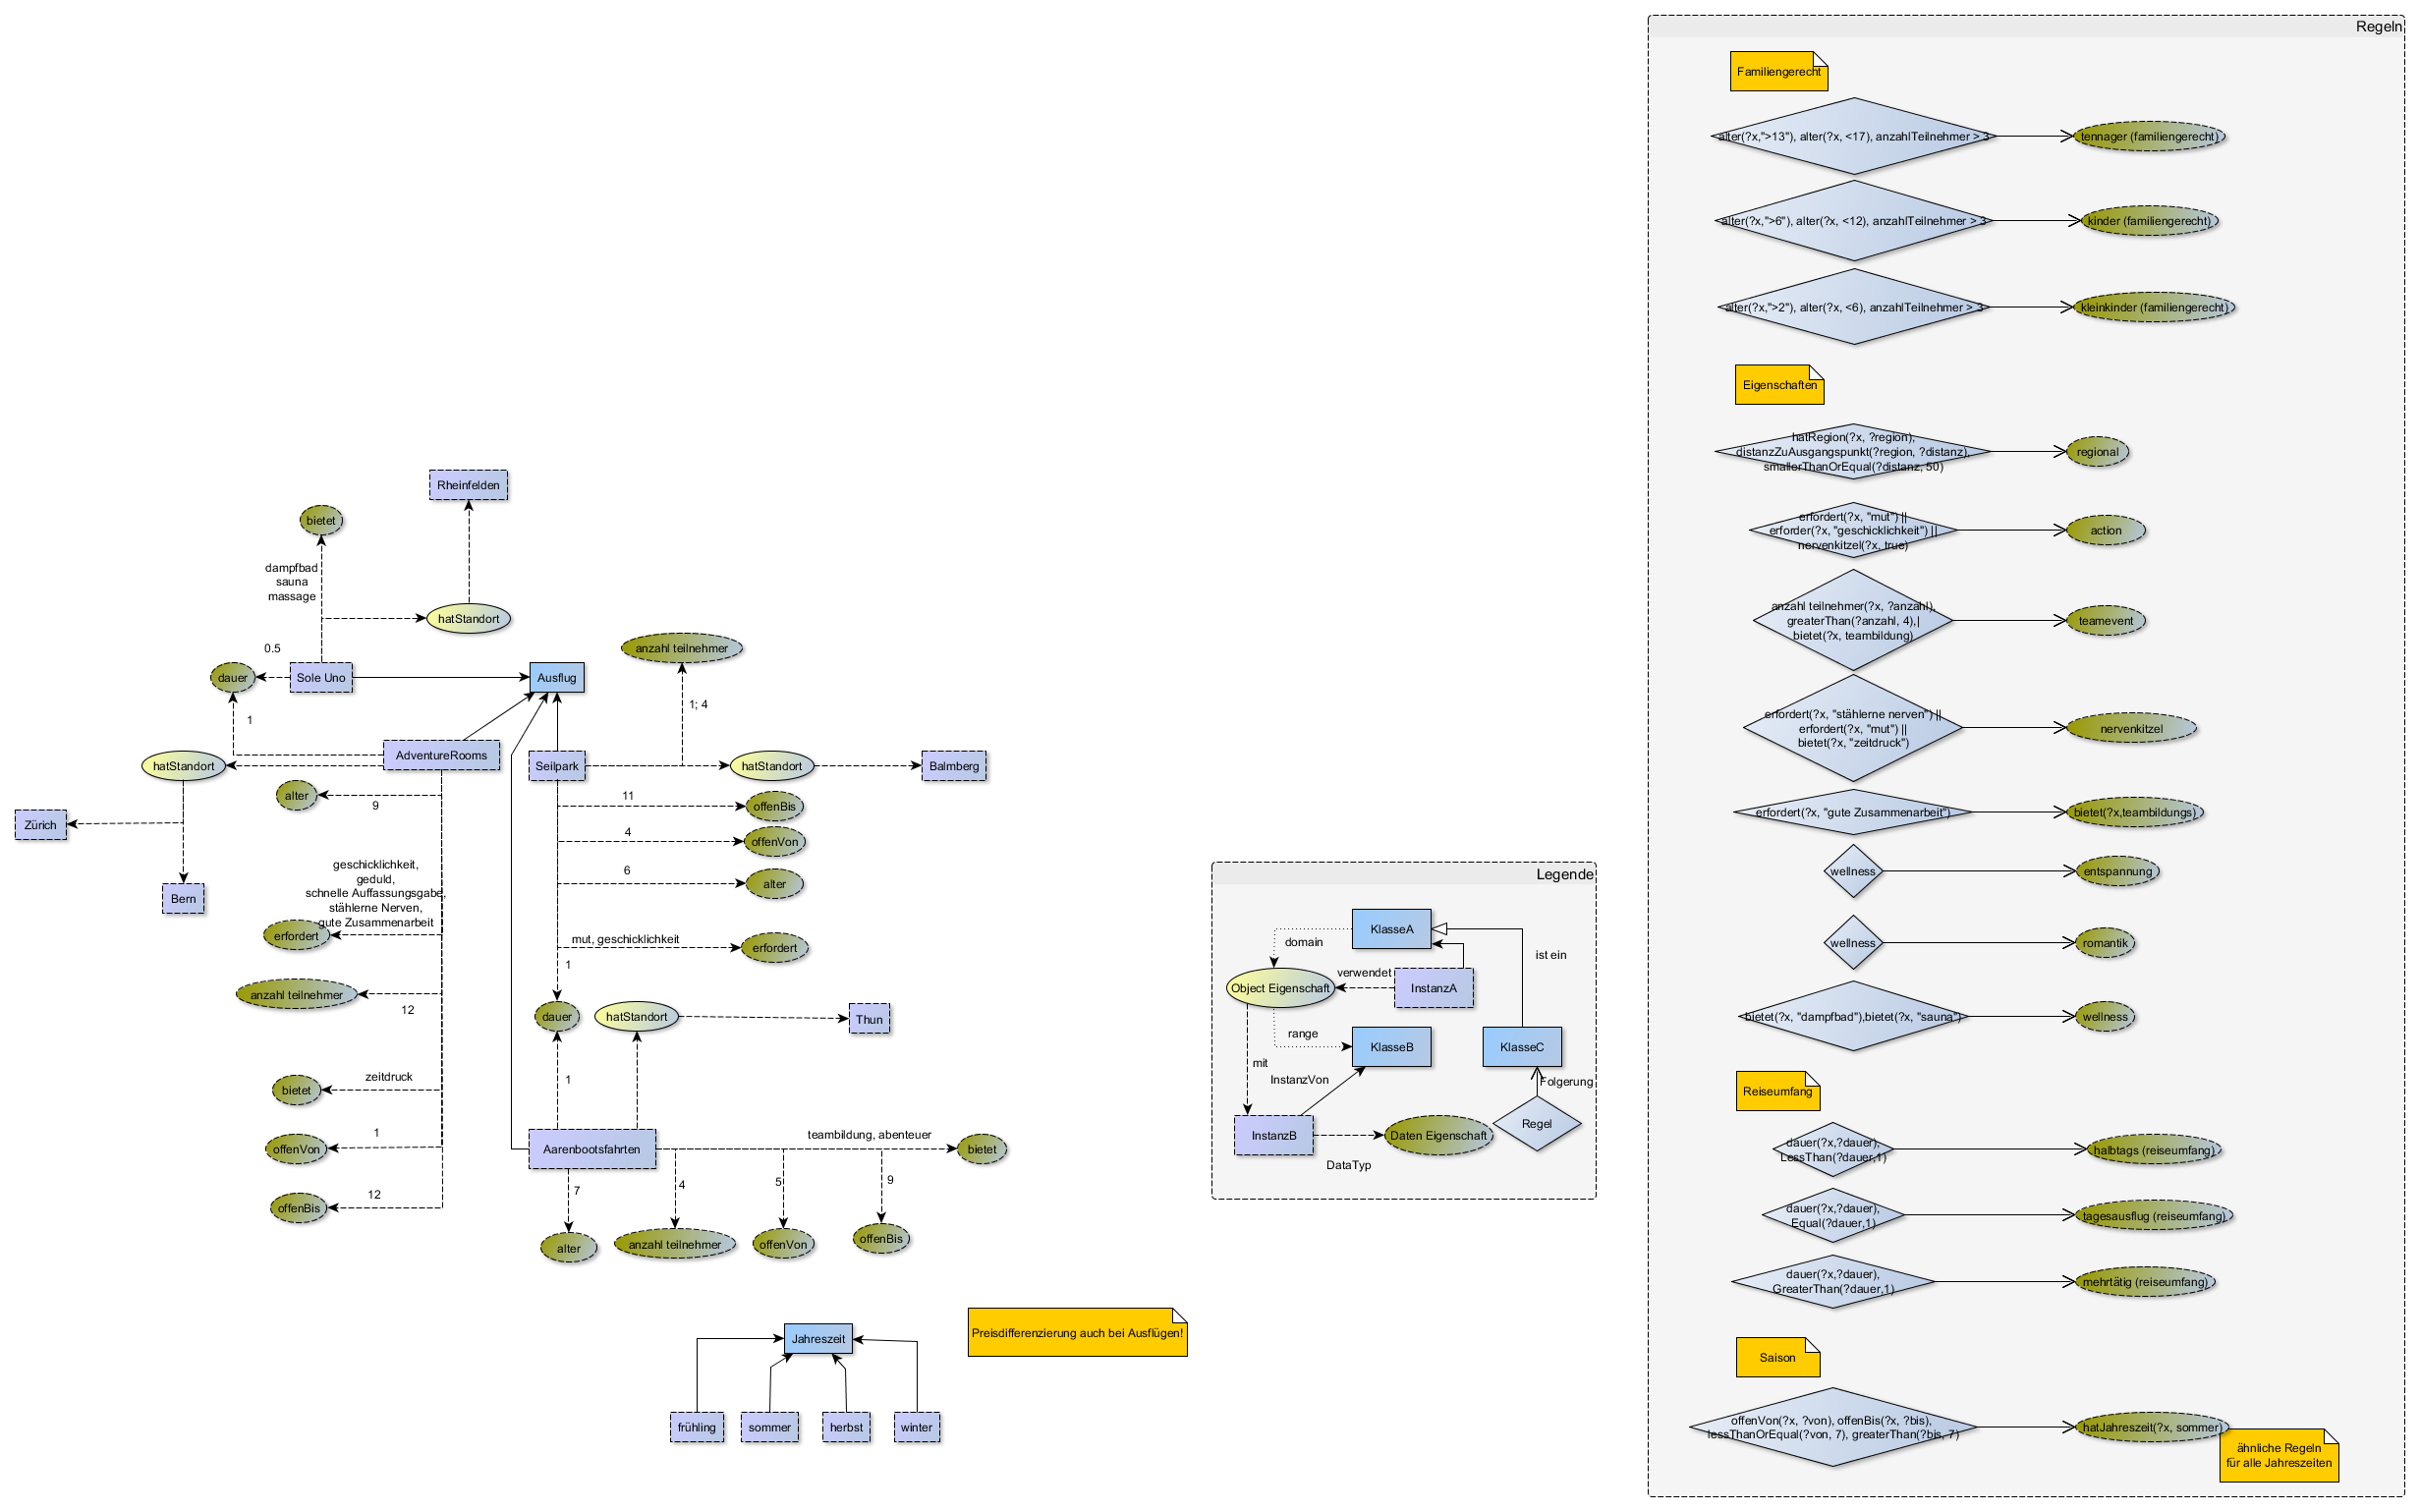
\includegraphics{bilder/semNetzLoesung.png}}}
\caption{Ausschnitt des semantischen Netzes zur Abbildung der Ontologie.\label{fig:semNetzLoesung}\protect\footnotemark}
\end{figure}
\footnotetext{Eigene Darstellung mittels yEd.}


Durch die Beschränkung der Problemdomäne auf Tages- und Wochenendausflüge in der Schweiz, konnten zwei Hauptkomponenten (Ausflüge und Restaurants) extrahiert werden.

Sowohl ein Restaurant als auch ein Ausflug werden durch Eigenschaften von Bedingungen (Bedingungsproperty) beschrieben. Ein Restaurantbesitzer könnte also dem Betreiber des erstellten Reiseplaners die Qualitäten seines Restaurants angeben. Diese Eigenschaften gehen von der Beschreibung des Ambientes, über kulinarischen Spezialitäten zu den durchschnittlichen Preisen, welche das Restaurant hat. Der Ausflug ist durch andere Werte wie der Anzahl Teilnehmer, den Öffnungszeiten oder was ein Ausflug bietet oder erfordert beschrieben.
Mittels Regeln ist festgelegt welche Folgerungen aus diesen Eigenschaften abgeleitet werden können.

Um die verschiedenen Möglichkeiten beim Abbilden einer Ontologie aufzuzeigen, wurde für die Spezifikation der Hauptkomponenten jeweils eine andere Umsetzung gewählt. Die Klasse Restaurant hat verschiedene Unterklassen. Der Besucher hat also bei der Suche die Auswahl zwischen verschiedenen Typen von Restaurants zur Verfügung. Je nach gewähltem Typ müssen unterschiedliche Kriterien (Bedinungsproperties) erfüllt sein. So ist zum Beispiel festgelegt, dass eine raffinierte Küche mit frischen und saisonalen Speisen auf ein Gourmetrestaurant schliessen lässt.

Wenn also in diesem Fall der Benutzer auswählt, dass er ein Gourmetrestaurant sucht, würden nur jene Restaurants ermittelt, welche als Eigenschaften raffinierte Küche mit frischen und saisonalen Speisen aufweisen. Das Preissegment ist als Klasse mit Individuen definiert. Jedes Individuum stellt da bei ein Preissegment dar. Liegt der Durchschnittspreis eines Restaurants in einem bestimmten Rahmen so definieren Regeln in welchem Preissegment das Restaurant liegt.  Dies ist durch eine Eigenschaft des Objektes (ObjectProperty) festgelegt. Objekteigenschaften beschreiben die Beziehungen zwischen zwei Individuen.

Bei den Ausflügen werden dem Benutzer des Reiseplaners Schlussfolgerungen angeboten. Mittels der vorher erwähnten Regeln ist festgelegt welche Bedienungen zutreffen müssen um eine gewisse Eigenschaft zu erfüllen. So ist zum Beispiel festgelegt, dass ein Ausflug der Wellness bietet entspannend und romantisch ist.\\
Sowohl Folgerungen als auch Bedingungen werden in Form von so genannten DataProperties definiert. Diese legen eine Eigenschaft eines Individuums fest.

In beiden Fällen ist zu beachten, dass der Benutzer sich entscheiden kann, ob er entweder eine von der Region oder von dem Ort abhängige Einschränkung für die Suche festlegen möchte. Die Beziehung zwischen den Region/Orten und den konkreten Ausflügen/Restaurants wird mit Hilfe von ObjectProperties erreicht. Es wird also zum Beispiel gesagt, dass ein Ausflug den Standort Bern hat. Als Erweiterung kann der Benutzer festlegen, dass er ein Restaurant sucht, welches sich im gleichen Ort respektive in der gleichen Region befindet wie der Ausflug.

Eine Besonderheit von Ausflügen ist, dass sie nicht das ganze Jahr über machbar sind. Durch eine Eigenschaft eines Ausfluges (DataProperty) kann der Betreiber festlegen in welchem Zeitraum ein Ausflug machbar ist (offen von bis).Dank geeigneter Regeln wird abgeleitet in welcher Saison ein Ausflugsziel besuchbar ist.

Eines der grösseren Probleme bei der Modellierung war die zeitliche Beschränkung. Bekanntlich kann dem Lösen von Planungsproblemen, welche NP-vollständig sind, eine ganze Bachelor Thesis gewidmet werden. Erschwerend kommt dazu, dass es bei der Wissensabbildung mittels OWL nur in sehr begrenztem Rahmen möglich ist zu rechnen. Da dies kein wichtiger Teil der Arbeit ist, haben die Autoren entschieden, dass es keinen Sinn macht diese Problematik in Form von Programmlogik zu lösen. Aus diesem Grund fällt die Zeitplanung relativ simpel aus. Es kann festgelegt werden wie viel Zeit ein Ausflug in Anspruch nimmt. In der Verwendung kann der Benutzer des Reiseplaners angeben wie viel Zeit er für einen Ausflug zur Verfügung hat. Zur Auswahl stehen die Kriterien halbtags, ganztags und mehrtägig, wobei die mehrtägigen Ausflüge nicht eingearbeitet wurden. In dieser Version des Reiseplaners werden in der Anfrage immer nur jene Ausflüge ausgegeben, welche der festgelegten Zeiteinheit entsprechen.

\subsection{Technische Schwierigkeiten}
\label{subsec:loesung_modellierung_technischeSchwierigkeiten}
TODO: evt doch in kapitel Technologien verschieben?!\\
Im Laufe der Modellierung sind die Autoren auf ein für sie unerklärliches Phänomen gestossen. So war es dem Reasoner in Stardog nicht möglich von einer DataProperty mit einem Wert auf die gleiche DataProperty zu schliessen. Konkret wollten die Autoren aussagen, dass ein Ausflug der eine Sauna bietet auch Wellness bietet. Diese Regel kann aber von Stardog nicht ausgewertet werden. Im Entwicklungstool Protégé wird die Schlussfolgerung aber richtig angezeigt. Nach längeren Recherchen entschieden die Autoren das es sich bei dieser Einschränkung wohl um einen technischen Fehler von Stardog handeln muss. Dies war doch sehr verwirrend, da beide Werkzeuge den gleichen Reasoner (Pellet) verwenden. Nach dem Buckreporing in der Stardogcommunity erhielten die Autoren die Information, dass es sich tatsächlich um einen Fehler im System handelt. Anscheinend wurde ein zu strenges Ausschlussverfahren in der Programlogik angewendet. Dieser soll aber im nächsten Release korrigiert werden. \\
Also Work-Arount wurde die Modellierung von den Autoren so umgebaut, dass Wellness ein DataProperty vom Type Boolean ist. Da es sich so nicht mehr um die gleiche DataProperty handelt, funktioniert die angepasste Regel.

\subsection{Output}
\label{subsec:loesung_modellierung_output}
Ein Teil des Outputs der Modellierung sind die oben erwähnten Semantischen Netze. Diese wurden in drei Grafiken aufgeteilt. Auf der ersten Grafik wird die gesamte Region/Ort Problematik abgebildet. Auf je zwei weiteren Grafiken wurden die Details zu den Restaurants respektive Ausflügen dargestellt.

Der zweite Teil ist ein durch das Entwicklungswerkzeug automatisch generierte RDF \ XML Dokument. Darin ist die Semantische Datenbank im OWL Format abgelegt. Es handelt sich dabei um die konkreten Daten.

\section{Generieren von Abfragen}
\label{sec:loesung_sparql}

Sowohl während des Abbilden der Problemdomäne als auch für die endgültige Suche mussten immer wieder Abfragen generiert werden. Dies geschieht in einer semantischen Datenbank mittels sparql Abfragen. Bei Spargl handelt es sich um eine  Abfragesprache für Ontologien todo ref Tutorial. Die Abfragen sind direkt in der Benutzeroberfläche integriert. So konnte verhindert werden, dass der Leser der Arbeit gezwungen ist, sich die Sprache anzueignen um die Suche zu benutzten.


\section{Benutzeroberfläche}
\label{sec:gui}

Nun sind alle oben beschriebenen Anforderungen abgedeckt. Eine letzte Aufgabe, die bis zu diesem Punkt noch unterschlagen wurde lautet "`...Besondere Bedeutung kommt dabei der Schnittstelle zwischen Mensch und System zu..."'. Nachdem klar wurde, dass es in keiner weise Benutzerfreundlich ist, Abfragen mittels Sparql selber zu schreiben, haben die Autoren entschieden eine Benutzeroberfläche zu implementieren. Dabei wird der Benutzer des Reiseplaners mit Hilfe eines Assistenten durch die Auswahl geführt. Neben der Vermeidung von Sparql während der Benutzung, ist so sichergestellt das der Benutzer nur Abfragen stellen kann, welche wenigstens in der Theorie Sinn ergeben. 
In einem ersten Schritt kann der Besucher entscheiden ob er nur ein Ausflug planen will, oder auch nach einem Restaurant sucht. Im zweiten Schritt werden sämtliche Folgepropertys zu den gewählten Komponenten angeboten. Zum Schluss erhält der Benutzer eine Liste sämtlicher Ergebnisse. Dabei wird aus allen gewählten Folgepropertys dynamisch eine Sparqlabfrage generiert. In der Outputliste sind der Name des Ausflugs, sein Standort und wenn vorhanden die URL zu seiner Homepage aufgelistet. Je nach Kriterienliste ist es natürlich möglich, dass keine Reise gefunden wird. Dies ist der Fall, wenn keine der erfassten Reisen auf die gewählten Kriterien passt. Da nur sehr exemplarisch Reisen erfasst wurde ist das Risiko für eine leere Antwort relativ hoch.

TODO: wo wollen wir die Architektur unsere Bentuezroberfläche hinmachen?

